\chapter{Introduction}
With the ongoing digital transformation it seems only a matter of time until the shift from paper based ballots will be replaced with electronic voting (e-voting). Recent polls show that the majority of the Swiss population is interested in having the possibility to vote online \footnote{\url{https://www.swissinfo.ch/ger/umfrage_grosse-zustimmung-zu-e-voting-trotz-sicherheitsbedenken/42457426}}. However, e-voting is a very complex topic and designing a secure e-voting protocol is known to be notoriously challenging in terms of IT-security and cryptography.

\section{Electronic voting}
First trials with e-voting in Switzerland date back to 2003. Since 2015, it is possible for Swiss citizens registered in the cantons Geneva and Neuchâtel and living abroad, to vote electronically. These systems were available only for a limited electorate size since they did not yet meet the requirements in terms of security and transparency, to be accepted as a secure E-Voting platform on a nationwide scale.

An e-voting system must satisfy a large variety of security requirements set up by the government, including:

\begin{itemize}
	\item Fairness: It is not possible for any person (including the participating parties of an e-voting system) to learn the intermediate result or outcome of an election before the result has been officially tallied and published to a public board.
	\item Privacy: No one can find out information about a voters selection. This implies that a voters ballot must be encrypted before it leaves the voters client and until the election is tallied.
	\item Authenticity: All voters must be authenticated as eligible voters in order to cast a vote
	\item Soundness: Only valid votes are being tallied. If a voter selects more candidates than he is allowed or less than he is supposed to, the vote must not be counted.
	\item Robustness: An e-voting system detects cheating actors.
\end{itemize}

There exist many different concepts and e-voting protocols that cover most of these requirements. However, most of the existing solutions behave as some kind of black-box and keep the internals hidden, such that a voter cannot be sure, whether his vote has been recorded correctly and counted in the final result.

One of the requirements that is hardest to achieve is the \textbf{universal verification}: A good e-voting system must be transparent and allow an external person to verify, that every protocol participant has abided by the protocol and that all and only valid votes have been counted correctly.

Another common problem is the \textbf{insecure platform problem}: If a voters computer is affected by malware, the vote casting process is no longer under the voters control and the candidate selection could be possibly manipulated without the voters notice. It must be \textbf{individually verifiable} to every voter that his intended vote has been recorded, while at the same time, the voters privacy must still be ensured at all times.

If an e-voting system shall be available to more than 30\% or 50\% of the respective cantonal electorate, it must be both individually as well as universally verifiable.

\section{CHVote Protocol}
Some of the mentioned requirements might sound as a paradox at first. However, they can be solved by advanced cryptography. A contract was formed between the state of Geneva and the  Research Institute for Security in the Information Society (RISIS) of the Bern University of Applied Sciences to work out a new protocol which does meet the complex requirements set up by the Swiss government. In 2017, Rolf Haenni, Philipp Locher and Reto E. Koenig published the resulting specification document and a proof-of-concept has been successfully implemented by the State of Geneva. Geneva is currently developing a new version of their e-voting system with the name "`CHVote"', based on this specification. Other cantons, currently St. Gallen, Aargau, Bern and Lucerne have announced their interest in cooperating with Geneva and might use their system in future.

The CHVote specifications document is publicly available and describes not only the theoretical background and the algorithms, but also provides pseudo-code for the approximately 75 algorithms that are needed to implement their protocol.

In chapter 3, we will summarize the most important aspects of the CHVote specifications that required for better understanding our work.

\section{Project task}
An additional problem e-voting is confronted, is that understanding such a complex protocol isn't easy without good knowledge in cryptography and mathematics. This might be one of the reasons why many people still do not trust electronic voting systems.

In close consultation with the authors of the CHVote specification, we were looking for an interesting project for our bachelor thesis in the thematic field of e-voting. We decided to study the CHVote specification, implement the protocol and build an application that allows to get a hands-on experience with the Geneva e-voting system and that could be used to show and explain to an audience how the future of voting in Switzerland might possibly look like.

\begin{center}
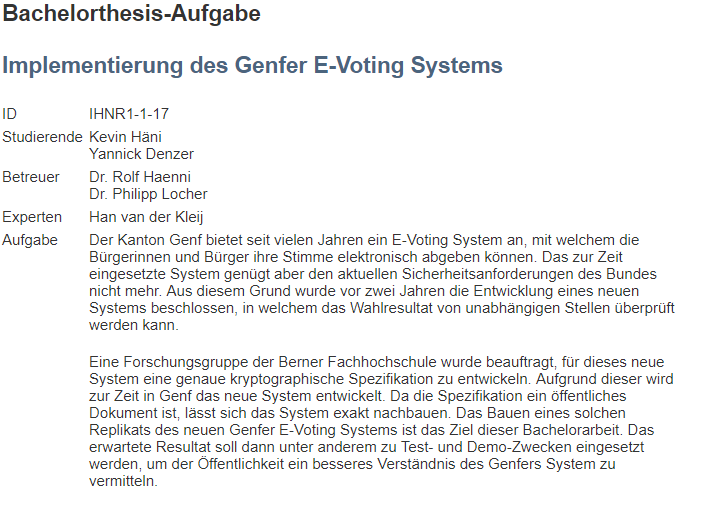
\includegraphics[scale=0.95]{assets/aufgabe.PNG}
\captionof{figure}{Bachelor thesis task}\label{Bachelor thesis task}%
\end{center}

Our project task required us to read and get a good understanding of the CHVote specification. As preparatory work during the course "`Project 2"', which we have finished just before the start of our bachelor thesis, we have implemented the approximately 65 algorithms which were defined as pseudo-code in the CHVote specification document. The resulting set of algorithms has been used as a library for implementing the protocol on which our application will be built on.

Based on this rather general task description, there were several possibilities regarding the final product, such as a realistic prototype, a verifier software for the implementation which is being developed in Geneva, or a demonstrator-application that targets the educational problem.

Ultimately we have decided for the last options: Our goal was to develop a web-based application that allows to visualize every step of a CHVote election event, from the pre-election tasks like generating the electorate data, to casting and confirming ballots from a voters point of view, to the post-election processes like mixing, decryption and tallying. Opposed to a realistic prototype, the focus on our project is not to implement an e-voting-system that is totally realistic and secure from an architectural perspective, but more on the visualization.

The authors of the specification have the intention of using our application for future demonstrations of their protocol to create a better understanding and acceptance for e-voting.

In chapter 2, we will further discuss the goals and requirements that we have set for this project. Additionally, it covers the time planing and project methodology of our project.

Chapter 3 will describe the final product and the concepts behind our application

Chapter 4 covers the technical aspects regarding the implementation, such as the architecture, the language and technology decisions. Later sections contain detailed information about the internals of each component of our application and the challenges we were facing during the implementation phase.

Chapter 5 will close this document with a short summary and a reflection about the project.
